\documentclass[11pt]{amsart}
\usepackage[margin=1.1in]{geometry}
\usepackage{amsmath,amssymb,amsthm}
\usepackage{booktabs}
\usepackage{tikz}
\usepackage[dvipsnames]{xcolor}
\usepackage{hyperref}
\hypersetup{colorlinks=true,linkcolor=blue!50!black,citecolor=blue!50!black,urlcolor=blue!50!black}
\def\UrlBreaks{\do\/\do-\do.}

\newtheorem{theorem}{Theorem}[section]
\newtheorem{lemma}[theorem]{Lemma}
\newtheorem{corollary}[theorem]{Corollary}
\theoremstyle{definition}
\newtheorem{definition}[theorem]{Definition}
\newtheorem{example}[theorem]{Example}
\theoremstyle{remark}
\newtheorem{remark}[theorem]{Remark}

\newcommand{\Z}{\mathbb{Z}}
\newcommand{\up}{{\uparrow}}
\newcommand{\ray}{\mathrm{ray}}

\title[Carriers, devices and fresh roots]{Carriers, devices and fresh roots:\\ the arrow method from minimum modulus 42 to 44}
% TODO(author): confirm name, affiliation and e-mail.
\author{Grayson MacKenzie}
\date{September 2026}

\begin{document}

\begin{abstract}
Nielsen and Owens constructed covering systems with distinct moduli whose smallest moduli are $40$ and $42$. They
filled ``holes'' prime by prime with arrows. We describe the ideas that carry this method to $44$. A capacity bound
decides which arrows can fit on a given piece of a hole. Carriers, congruences that cover whole slots of arrows in
other sections, can be routed to where they are needed by relabelling them modulo $5$. The unique family of smallest
modulus can be cut back to its deeper levels. The part of the integers that its first level alone covered is then
small, and an exact computation lists where it lies. We cover it again with roots on fresh primes, helped by a small
device on the prime $7$ whose digits serve as exact carries. For the second step we nest a smaller arrow into the slot
of the offending input. The thin remainder is closed by further roots and by local repairs found from exact
counterexamples.
\end{abstract}

\maketitle

\section{Introduction}

A finite set of congruence classes $a_i \bmod m_i$ with distinct moduli $m_i>1$ whose union is $\Z$ is a
\emph{covering system}. In 1950 Erdős \cite{Erdos50} asked whether the smallest modulus of a covering system can be
arbitrarily large. Filaseta, Ford, Konyagin, Pomerance and Yu \cite{FFKPY07} restricted such systems severely, and
Hough \cite{Hough15} proved that the answer is no: the smallest modulus is at most $10^{16}$. Balister, Bollobás,
Morris, Sahasrabudhe and Tiba \cite{BBMST22} lowered the bound to $616{,}000$.

Constructions have come slowly. Churchhouse \cite{Churchhouse68} found a covering system with smallest modulus $9$ in
1968. In 1971 Krukenberg \cite{Krukenberg71} reached $18$ and Choi \cite{Choi71} $20$. About ten years later Morikawa
\cite{Morikawa81a,Morikawa81b} reached $24$, and Gibson \cite{Gibson09} then reached $25$. Nielsen \cite{Nielsen09}
introduced a compact notation for such constructions, built around \emph{arrows}, and reached $40$. Owens
\cite{Owens14} extended the method to $42$.

\begin{theorem}\label{thm:44}
There is a covering system with distinct moduli whose smallest modulus is $44$.
\end{theorem}

The system, $618{,}413$ families of congruences on the $47$ primes up to $211$, is given with its verification in the
companion paper \cite{Companion}. Here we explain how it was found, in the manner of \cite{Nielsen09} and
\cite{Owens14}: which hole we are filling, which sets are available, and how many sets we obtain. We start from a
system with smallest modulus $42$, a variant of Owens's (§\ref{sec:carriers}). We reach $43$ in
§§\ref{sec:cut}--\ref{sec:roots} and $44$ in §\ref{sec:44}. As far as we know, the following ideas are new.
\begin{itemize}
\item \emph{A capacity bound} (§\ref{sec:capacity}). It bounds how many pairwise separated covers a piece of the
  integers can hold, and so which primes can root an arrow there.
\item \emph{Exact censuses} (§\ref{sec:census}). Whether a region is covered is a finite question. A counterexample
  loop lists exactly where a hole lies and certifies that the list is complete.
\item \emph{Carrier routing} (§\ref{sec:carriers}). A few congruences cover whole slots of arrows in other sections.
  Relabelling such a carrier modulo $5$ decides which sections receive its carry.
\item \emph{Cutting back the smallest family} (§\ref{sec:cut}). The unique family of smallest modulus keeps its deeper
  levels and gives up only its first.
\item \emph{Devices} (§\ref{sec:device}). A few families on deep rays cover fixed digits exactly, and so serve as
  exact carries.
\item \emph{Fresh roots} (§\ref{sec:roots}). An arrow on a prime used nowhere else covers one piece of the hole.
  Its inputs are separated covers of that piece.
\item \emph{Nesting in the offending slot} (§\ref{sec:44}). The input responsible for the smallest modulus is
  replaced by an arrow on a smaller prime. Every other input stays in its slot.
\item \emph{Local repairs} (§\ref{sec:44}). Each uncovered point that the exact computation returns is traced to the
  input that misses it, and that input is patched in place.
\end{itemize}

\section{Notation}\label{sec:notation}

We follow Nielsen \cite[§2]{Nielsen09}. For a prime $q$, the expression $q(A_1,\dots,A_q)$ denotes the congruences
obtained by placing the set $A_j$ on the branch $j \bmod q$. Each set is scaled by $q$: an entry $m$ on branch $j$
stands for a congruence class of modulus $qm$ inside $j \bmod q$. The \emph{arrow} is the infinite recursion
\[
q\up(A_1,\dots,A_{q-1}) = q\bigl(A_1,\dots,A_{q-1},\,q\up(A_1,\dots,A_{q-1})\bigr).
\]
The same $q-1$ \emph{inputs} are reused on every level, deeper and deeper inside $0 \bmod q$. The input $A_j$ thus
covers, inside the region, the integers $x\ne0$ whose first nonzero digit in base $q$ is $j$. We call this set the
\emph{slot} $j$ of the arrow, and the digit its \emph{$q$-lead}. For example, in $3\up(1,2\up)$ the first input
contributes the class $3^{k-1} \bmod 3^k$ on every level $k$. The second contributes $2\cdot 3^{k-1} \bmod 3^k$,
intersected with the congruences of $2\up$ \cite[Example~1]{Nielsen09}. Nielsen stops the recursion at a deep level
and covers what is left with the help of a large auxiliary prime. At a deep enough level every modulus this introduces
is large, and distinct powers keep the moduli distinct.

For bookkeeping we write the congruences produced by one path through the arrows as a \emph{family}: a product over
primes of \emph{coordinates}. A coordinate is either \emph{fixed}, one class $r \bmod p^e$, or a \emph{ray}
$\ray(p,[\ell,h],c,d)$: the classes $c+d\,p^{e-1} \bmod p^e$ for $\ell\le e\le h$ (we allow $h=\infty$). The number
$c$ is the ray's \emph{centre}. A family's moduli are the products of one prime power per coordinate, and its
\emph{box} is the product of its exponent ranges. Two families can repeat a modulus only if they involve the same
primes and their boxes overlap. When no two families of a collection do this, we call the collection
\emph{separated}.

Two conventions of Owens \cite{Owens14} matter below. First, an input of multiplier $\mu$ in a $q$-arrow gives a
first-level modulus $q\mu$. It is therefore allowed only if $q\mu\ge N$, where $N$ is the target smallest modulus. For
$N=42$, for instance, the inputs $1$ and $2$ must be dropped from a $19$-arrow. Second, a slot is \emph{carried}
where earlier material already covers it, and a carried slot needs no input there.

We refer to the sections of the construction by their numbers in \cite{Owens14}. For instance, §3.4 is the section of
the prime $7$, §3.5 that of $11$ and §3.14 that of $43$. A \emph{cell} is a set of the form
$\{x : v_2(x)=k,\ x\equiv r \bmod 5\}$ inside a fixed residue class, written $(k,r)$. A \emph{piece} is a cell further
restricted by one or more leading digits.

\section{Two tools}\label{sec:tools}

\subsection{A capacity bound}\label{sec:capacity}

Much of what follows is a question of whether a piece of the integers has room for $q-1$ separated covers. The
following bound answers it in the negative surprisingly often.

\begin{lemma}\label{lem:capacity}
Let $Q$ be a finite set of primes. Let $R$ be a residue class modulo $\prod_{p\in Q}p^{a_p}$, where $a_p\ge0$. Let
$T_1,\dots,T_n$ be sets of congruence classes with $Q$-smooth moduli, each covering $R$, and suppose that no modulus
occurs twice among all of them. Then
\[
n \;\le\; \nu(R) \;:=\; \prod_{p\in Q}\Bigl(a_p+1+\frac{1}{p-1}\Bigr).
\]
If every modulus is at least $t$, then more precisely
$n\le\sum_{m\ge t}\prod_{p\in Q}\min\bigl(1,p^{a_p-v_p(m)}\bigr)$, the sum running over the $Q$-smooth $m\ge t$.
\end{lemma}

\begin{proof}
A class of modulus $m$ meets $R$ in a class modulo $\operatorname{lcm}(m,\prod p^{a_p})$, or not at all. Its share of
$R$ is therefore at most $w(m)=\prod_p \min(1,p^{a_p-v_p(m)})$. Since $T_i$ covers $R$, the shares of its classes add
up to at least $1$. Summing over $i$ and using that the moduli are distinct gives $n\le\sum_m w(m)$. Without the
restriction $m\ge t$ the sum factors as
$\prod_p\sum_{e\ge0}\min(1,p^{a_p-e})=\prod_p\bigl(a_p+1+\tfrac1{p-1}\bigr)$.
\end{proof}

An unpinned prime contributes the factor $p/(p-1)$. A computation of the same kind shows that a piece pinned by a
single leading digit at $p$, on every level, gets the factor $2$. A root on $q$ over $R$ with $c$ carried slots needs
$q-1-c$ inputs that cover $R$ and do not repeat each other's moduli once the factor $q$ is removed. So it fits only
if $q-1-c\le\nu(R)$, computed without the prime $q$. The bound is also nearly attained in practice.

\begin{remark}\label{rem:tight}
Measured against this bound, the construction of Owens is nearly tight. Each of its sections needs between $93\%$
and $100\%$ of $\nu$ for its root (median about $96\%$). Our starting system spends $94.7\%$ of the sum $3.830$ of
$1/m$ over the $83$-smooth $m\ge42$. So every gain has to come from new room: fresh primes, or lattice points that no
family uses.
\end{remark}

\subsection{Exact censuses}\label{sec:census}

Everything below depends on knowing exactly where a hole is. This is possible because coverage is a finite question.

\begin{lemma}\label{lem:atoms}
Let $F$ be a finite set of families. For each prime $p$ involved there is a partition of $\Z$ into finitely many
\emph{atoms} such that every coordinate of $F$ on $p$ is a union of atoms, and every atom is either a single ray
centre or contains a full residue class modulo a power of $p$. Hence whether an integer is covered by $F$ depends
only on the atoms that contain it. Every choice of one atom per prime, none of them a centre, is realised by
infinitely many integers.
\end{lemma}

\begin{proof}
Take $E$ larger than every finite exponent in $F$ and than $v_p(c-c')$ for any two distinct centres $c,c'$ on $p$.
The atoms are the classes modulo $p^E$ that contain no centre. The class of each centre $c$ is split into the point
$c$ and, for $j=1,\dots,p-1$, the integers $x\ne c$ in it whose leading digit of $x-c$ is $j$. A fixed coordinate
of exponent less than $E$ is a union of classes modulo $p^E$. A ray $\ray(p,[\ell,h],c,d)$ consists of the $x$
with $\ell-1\le v_p(x-c)\le h-1$ and leading digit $d$, so it is a union of atoms as well. The atom with leading digit
$j$ contains the class $c+jp^E \bmod p^{E+1}$. The last claim follows from the Chinese remainder theorem.
\end{proof}

So whether a region $X$ is covered is the satisfiability question for a propositional formula. It has one variable
per atom and one clause per family, which says that the point is not in that family. It also has clauses saying that
the point takes exactly one atom per prime and lies in $X$. The formula is unsatisfiable if and only if $X$ is
covered, and a solver such as CaDiCaL \cite{CaDiCaL} gives a proof of unsatisfiability that can be checked
independently \cite{DRATtrim}. A satisfying assignment that avoids the centres decodes into an explicit uncovered
integer.

We use this in two loops. In a \emph{census}, each counterexample is widened to the piece that contains it: its
atoms at a few small primes, and its leading digit at the root prime of the section that owns it. That piece is
blocked, and we ask again. When the formula becomes unsatisfiable, the blocked pieces contain the whole hole, and
the final proof certifies that the list is complete. In a \emph{repair}, each counterexample is instead traced to the
input that should have covered it, that input is patched, and we ask again (§\ref{sec:44}).

\section{Carrier routing and the starting system}\label{sec:carriers}

In the sections for $11$, $13$ and $17$ (§§3.5--3.7) a few bare congruences do more than their own job. They cover a
whole slot of an arrow used much later, on an even branch. We call these congruences \emph{carriers}. Each one lies
in a single class modulo $5$, and that class is a digit of its own $5$-arrow. The later sections live in different
classes modulo $5$, so the label of a carrier decides which of them receive its carry. The three that carry a whole
slot are listed in Table~\ref{tab:carriers}, where $q{:}j$ is the slot of digit $j$ in the $q$-arrows of the
receiving sections.

\begin{table}[ht]
\centering
\caption{The whole-slot carriers of §§3.5--3.7 and the later sections that receive their carry, by label.}\label{tab:carriers}
\begin{tabular}{@{}lllll@{}}
\toprule
carrier & modulus & slot & label & sections receiving the carry\\
\midrule
$C_{55}$ & $55$ & $11{:}6$ & $1$ & §§3.8, 3.12, 3.17\\
         &      &          & $4$ & §§3.14, 3.15, 3.16, 3.18, 3.20\\
$C_{65}$ & $65$ & $13{:}6$ & $2$ & §§3.10, 3.13, 3.19\\
         &      &          & $4$ & §§3.14, 3.15, 3.16, 3.18, 3.20\\
$C_{85}$ & $85$ & $17{:}9$ & $1$ & §§3.8, 3.12, 3.17\\
         &      &          & $4$ & §§3.14, 3.15, 3.16, 3.18, 3.20\\
\bottomrule
\end{tabular}
\end{table}

A carried slot is worth one whole input to the arrow that receives it, so moving a carrier moves one input from one
section to another. Here is how we used this. Give $C_{55}$, $C_{65}$ and $C_{85}$ the labels $1$, $2$ and $1$. The $67$-arrow of §3.18
then finds only $63$ of the $64$ sets of its own that it needs. The other two of its sixty-six inputs come, as in
\cite{Owens14}, from doubling. There are two ways to give that arrow a whole slot.
\begin{itemize}
\item \emph{Move $C_{65}$ to label $4$.} The $67$-arrow then reaches $64$. But §3.19 uses $13$-arrows with only
  eleven inputs, because their slot $6$ is carried there. Without the carry, both halves of §3.19 fall eight inputs
  short.
\item \emph{Move $C_{85}$ to label $4$.} The $67$-arrow again reaches $64$. The sections that lose the carry do not
  need it: §3.8 still builds its twenty sets, and §§3.12 and 3.17 still close.
\end{itemize}
So we move $C_{85}$. Concretely, its $5$-arrow in §3.7 is written $5\up(8\up,2,4,1)$ instead of $5\up(1,2,4,8\up)$.
The remaining arrangement is done by an exact planner. For each section, a dynamic programme over subsets of the
available base sets chooses the order in which the arrows are built. It re-plans §§3.12, 3.14 and 3.15 and both
arrows of §3.18, and §3.18 needs no $89$-arrow. We call the result UC85. It has $356{,}364$ families on the $23$
primes up to $83$, and its smallest modulus $42$ is attained exactly once.

\section{Cutting back the smallest family}\label{sec:cut}

The modulus $42=2\cdot3\cdot7$ comes from one family of §3.4,
\[
F_{42} = \{0 \bmod 2\}\cdot\{1 \bmod 3\}\cdot\ray(7,[1,\infty),0,3),
\]
whose first level is the class $10 \bmod 42$. To reach $43$ we start its ray one level lower, at
$\ray(7,[2,\infty),0,3)$. The moduli $2\cdot3\cdot7^e$ with $e\ge2$ remain, and only the class $10 \bmod 42$ is
given up (Figure~\ref{fig:cut}).

\begin{figure}[ht]
\centering
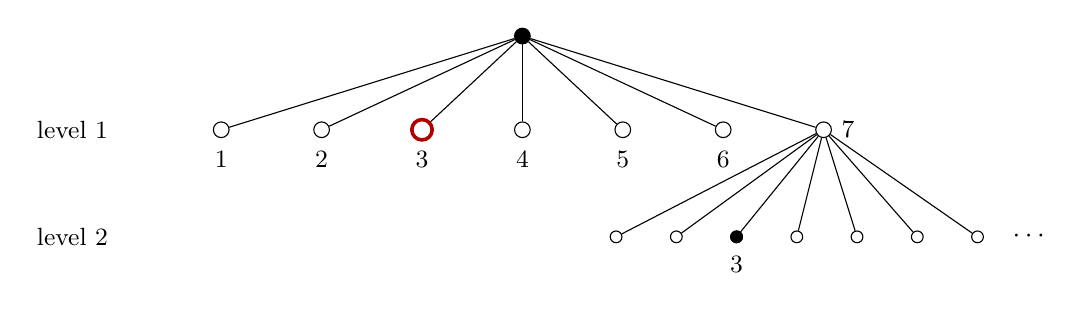
\begin{tikzpicture}[scale=0.85]
  \node[circle,draw,fill=black,inner sep=2pt] (r) at (0,0) {};
  \foreach \j/\x in {1/-4.5,2/-3,3/-1.5,4/0,5/1.5,6/3,7/4.5} {
    \node[circle,draw,inner sep=2pt] (b\j) at (\x,-1.4) {};
    \draw (r) -- (b\j);
  }
  \foreach \j/\x in {1/-4.5,2/-3,3/-1.5,4/0,5/1.5,6/3} \node[below=2pt] at (\x,-1.5) {\small \j};
  \node[right=3pt] at (4.5,-1.4) {\small 7};
  \node[circle,draw=red!70!black,fill=white,inner sep=2.6pt,line width=1.3pt] at (-1.5,-1.4) {};
  \foreach \j/\x in {1/1.4,2/2.3,3/3.2,4/4.1,5/5.0,6/5.9,7/6.8} {
    \node[circle,draw,inner sep=1.5pt] (c\j) at (\x,-3.0) {};
    \draw (b7) -- (c\j);
  }
  \node[circle,draw,fill=black,inner sep=1.5pt] at (3.2,-3.0) {};
  \node[below=1pt] at (3.2,-3.1) {\small 3};
  \node at (7.6,-3.0) {$\cdots$};
  \node[anchor=west] at (-7.4,-1.4) {\small level $1$};
  \node[anchor=west] at (-7.4,-3.0) {\small level $2$};
\end{tikzpicture}
\caption{The $7$-tree of $F_{42}$ on the branch $\{0 \bmod 2\}\cap\{1 \bmod 3\}$. Branch $7$ is $0 \bmod 7$, where the
tree recurs. The ray covers the digit $3$ on every level. Cutting it back gives up only the outlined first-level
class, $10 \bmod 42$; the filled class and its copies further down are kept.}\label{fig:cut}
\end{figure}

Most of $10 \bmod 42$ is still covered by other families. What is left, the hole $U$, is about $2.1\%$ of the class,
or $4.95\cdot10^{-4}$ of the integers. Every integer in $10 \bmod 42$ is even and $\equiv 3 \bmod 7$. Sorting by
$v_2(x)$ and $x \bmod 5$, an exact census (§\ref{sec:census}) shows that $U$ meets exactly fourteen cells.
Table~\ref{tab:hole} lists them with their sizes, which were estimated by sampling.

\begin{table}[ht]
\centering
\caption{The hole $U$ after cutting back $F_{42}$: the uncovered fraction of each cell $(v_2(x),\,x \bmod 5)$ of
$10 \bmod 42$ (sampled). A dash marks a cell that $U$ does not meet; $U$ also contains no multiple of $32$.}\label{tab:hole}
\begin{tabular}{@{}lccccc@{}}
\toprule
$v_2 \backslash\, x \bmod 5$ & $0$ & $1$ & $2$ & $3$ & $4$\\
\midrule
$1$ & $0.14\%$ & $0.65\%$ & $0.80\%$ & $1.58\%$ & $0.62\%$\\
$2$ & $0.41\%$ & $2.21\%$ & $6.65\%$ & $8.66\%$ & $5.36\%$\\
$3$ & -- & -- & $7.85\%$ & $10.2\%$ & $5.40\%$\\
$4$ & -- & -- & -- & -- & $2.49\%$\\
\bottomrule
\end{tabular}
\end{table}

The hole has two sources. Where $v_2(x)\ge2$ it is mostly the part of $10 \bmod 42$ that $F_{42}$ alone covered. The
row $v_2=1$ and the cells $(2,1)$ and $(4,4)$ come from carries that $F_{42}$ had supplied to arrows of later
sections: §§3.16, 3.8, 3.10, 3.10 and 3.15 for $(1,0),\dots,(1,4)$, §3.12 for $(2,1)$ and the $79$-arrow of §3.20
for $(4,4)$. For instance, on the cell $(1,1)$ the hole lies only in the $19$-slots $16$, $17$ and $18$. These are the
three copies of $7\up$ in §3.8, whose slot $3$ was carried by $F_{42}$. The holes in $(1,0)$ and $(2,0)$ lie in
$20 \bmod 25$.

One might hope to re-plan the sections that lose a carry. This fails. With $F_{42}$ cut back, §3.8 reaches $19$ of its
$20$ sets, §3.10 $27$ of $28$, §3.12 $34$ of $36$, §3.15 $44$ of $46$ and §3.16 $48$ of $52$. The $67$-arrow of
§3.18 falls to $65$ of $66$. A section that is short leaves a whole root slot open on its whole region, which is far
worse than $U$. So we keep the sections as they are and cover $U$ from outside.

\section{A device on the prime 7}\label{sec:device}

The whole hole lies in $3 \bmod 7$, where $7$ divides $x+4$. Write $R_j=\ray(7,[2,\infty),-4,j)$. Inside
$3 \bmod 7$, $R_j$ covers exactly the integers $x\ne-4$ for which the first nonzero digit of $x+4$ in base $7$ is $j$.
We use the seven families
\begin{gather*}
\{0 \bmod 2\}R_1,\quad \{1 \bmod 3\}R_2,\quad \{0 \bmod 4\}R_3,\quad \{0 \bmod 4\}\{13 \bmod 27\}R_4,\\
R_5,\quad \{3 \bmod 5\}R_6,\quad \{24 \bmod 32\}\{1 \bmod 3\}\{2 \bmod 5\}R_6.
\end{gather*}
Their smallest moduli are $98$, $147$, $196$, $5{,}292$, $49$, $245$ and $23{,}520$. No other family of the system
has the same primes and an overlapping box, so they cost nothing. The ray $R_5$, for instance, uses the pure powers
$7^e$, $e\ge2$, which no other family uses. Inside $10 \bmod 42$, which is even and $\equiv 1 \bmod 3$,
the device covers the leading digits $1$, $2$ and $5$ of $x+4$ everywhere. It also covers the digit $3$ on
$0 \bmod 4$, the digit $6$ on $3 \bmod 5$, and a little more.

We call such a small set of families a \emph{device}. By itself it covers about $70\%$ of $U$ but empties no cell,
since every cell contains every digit. Its value is that it is exact and uniform. Any cover of a piece that works deep
in the $7$-adic direction, with centre $-4$, may treat the device's digits as carried slots. On a cell with
$v_2=1$ these are the digits $1,2,5$. With $v_2\ge2$ the digit $3$ is added, and on $x\equiv3\bmod5$ the digit $6$.

\section{Fresh roots}\label{sec:roots}

Suppose a piece $P$ of the hole is to be covered by a $q$-arrow on a prime $q$ used nowhere else in the system. We
call this a \emph{fresh root}. Every congruence of the root carries a power of $q$, so the root cannot repeat a
modulus of any family outside it. It needs $q-1$ inputs, each a set of congruences covering $P$, and the inputs must
be separated from one another. By Lemma~\ref{lem:capacity} this is possible only if $q-1\le\nu(P)$, less the carried
slots. We call the largest number of separated covers of $P$ that we can build its \emph{pool}. The building blocks
are fixed coordinates, deep rays on the pinned primes, and arrows on the primes from $11$ upwards, other than $q$.

Carried slots raise the pool, but only if they are carried exactly. We use two sources of exact carries: the digits
of the device, and the slots of a section's root that an exact computation proves covered on the piece. Carries
observed only on samples are not safe. On one cell with $v_2=1$ they suggested a pool of $156$, and the exact
computation showed that they did not hold. Table~\ref{tab:pools} shows the pools we reached.

\begin{table}[ht]
\centering
\caption{Pools of separated covers. \emph{Base}: covers made of fixed coordinates and rays only. \emph{Pool}: with
arrows. $\nu$: the bound of Lemma~\ref{lem:capacity} with the primes up to $200$. The last column uses exact carries.}\label{tab:pools}
{\small
\begin{tabular}{@{}lcccl@{}}
\toprule
piece & base & pool & $\nu$ & with exact carries\\
\midrule
cell, $v_2=1$ & $46$ & $74$ & $\approx105$ & $88$--$96$ (root digits, device); $122$ split mod $8$\\
cell, $v_2=2$ & $58$ & $104$ & $\approx133$ & $131$ (device digits $1,2,3,5$); $140$ on $(2,1)$\\
cell, $v_2=3$ & $70$ & $121$ & $\approx160$ & at least $148$ (device)\\
cell, $v_2=4$ & $83$ & $160$ & $\approx186$ & --\\
$(1,1)$, a $19$-digit pinned & $95$ & $177$ & $\approx202$ & --\\
$(1,0)$, $(2,0)$ in $20 \bmod 25$ & $68$ & $\ge126$, $\ge150$ & -- & --\\
\bottomrule
\end{tabular}}
\end{table}

The primes $11$ to $83$, which the construction already uses, cannot serve as roots. The sections that use them
occupy the low-lying lattice points, and a root on one of them would have room for at most seven covers. Two
principles then decide the assignment. First, the weakest cells, those with $v_2=1$, go on the smallest primes,
since a root on $q$ needs only $q-1$ inputs. Second, a cell whose pool falls just short is split, by $x \bmod 8$ or
by a leading digit, and each part gets a root of its own. Our first assignment, with twelve roots, the device and the
fills described below, left $48$ pieces uncovered. All of them lay in the cells $(1,2)$, $(1,3)$, $(1,4)$ and
$(2,1)$, at a few leading digits of the roots of §§3.10, 3.15 and 3.12. The same computation proves the other digits
of those roots covered on these cells. Used as exact carries, they are what made the final assignment of seventeen
roots work, and the final system is checked again as a whole.

\subsection*{The Prime 89}
We begin with the cell $(1,2)$: the part of $U$ with $x\equiv2 \bmod 4$ and $x\equiv2 \bmod 5$. It lies in the
region of §3.10, whose $29$-root covers nineteen of its twenty-eight slots on this cell (an exact computation shows
this). The device gives the $7$-digits $1$, $2$ and $5$. With these carries we obtain eighty-eight sets, which is
exactly what $89\up$ needs ($5{,}818$ families).

\subsection*{The Primes 97, 101 and 103}
The cell $(1,3)$ is handled in the same way, now also with the device digit $6$, since $x\equiv3 \bmod 5$ there:
ninety-six sets for $97\up$ ($16{,}972$ families). The cell $(1,4)$ lies in the region of §3.15. Its $47$-root covers
twenty-eight slots there, but even with that carry the cell is too large for one root. We split it by $x \bmod 8$,
covering $2 \bmod 8$ with $101\up$ and $6 \bmod 8$ with $103\up$.

\subsection*{The Primes 107 through 173}
The remaining cells are filled one root at a time, as listed in Table~\ref{tab:roots}. The cells with $v_2\ge2$ use the
device digit $3$ as well. The cell $(1,1)$, whose hole lies in three $19$-slots, is pinned further by its $19$-digit,
and each digit gets a root of its own.

\begin{table}[ht]
\centering
\caption{The seventeen fresh roots of the step to $43$. A cell $(v_2(x),\,x \bmod 5)$ is taken inside
$10 \bmod 42$; ``device'' lists the $7$-digits used as carries.}\label{tab:roots}
\small
\begin{tabular}{@{}rlll@{}}
\toprule
$q$ & piece & exact carries used & families\\
\midrule
$89$ & $(1,2)$ & $29$-root, $19$ slots; device $1,2,5$ & $5{,}818$\\
$97$ & $(1,3)$ & $29$-root, $19$ slots; device $1,2,5,6$ & $16{,}972$\\
$101$, $103$ & $(1,4)$ split by $x \bmod 8$ & $47$-root, $28$ slots; device $1,2,5$ & $3{,}280$, $4{,}728$\\
$107$ & $(1,0)$ in $20 \bmod 25$ & device $1,2,5$ & $2{,}052$\\
$109$, $113$ & $(2,2)$, $(2,4)$ & device $1,2,3,5$ & $4{,}508$, $7{,}898$\\
$127$, $149$ & $(2,3)$, $(3,3)$ & device $1,2,3,5,6$ & $6{,}181$, $3{,}006$\\
$131$ & $(2,1)$ & $37$-root, $24$ slots; device $1,2,3,5$ & $33{,}806$\\
$137$, $139$ & $(3,2)$, $(3,4)$ & device $1,2,3,5$ & $13{,}940$, $22{,}278$\\
$151$, $157$ & $(2,0)$ in $20 \bmod 25$, $(4,4)$ & device $1,2,3,5$ & $4{,}456$, $8{,}496$\\
$163$, $167$, $173$ & $(1,1)$, $19$-digits $16$, $17$, $18$ & device $1,2,5$ & $7{,}598$, $11{,}778$, $27{,}056$\\
\bottomrule
\end{tabular}
\end{table}

\subsection*{Filling slots in place}
Cutting back $F_{42}$ also leaves some copies of arrows in §§3.10, 3.12 and 3.15 with an empty slot. Where the lattice
had room, we filled such a slot directly. We used the slot's context times the class $1 \bmod 3$ (and $3 \bmod 7$ when
needed), with a coordinate on $2$ or $5$ added when that made the modulus new. This adds $3$, $75$ and $526$ families
to the three sections. It helps, but most contexts are already saturated by the sections' own base rays ($8\up$,
$9\up$ and $25\up$), so fills alone cannot replace the roots.

With the device, the fills and the seventeen roots, the class $10 \bmod 42$ is covered again. The system now has
$540{,}826$ families on the $40$ primes up to $173$. Its smallest modulus $43$ is attained once, by the input $1$ of
the $43$-arrow of §3.14, and each of the moduli $43$ to $48$ occurs once.

\section{From 43 to 44}\label{sec:44}

The modulus $43$ comes from the input of multiplier one of the root $43\up$ of §3.14. This is the bare family
$\ray(43,[1,\infty),0,1)$, which covers the $43$-lead $1$ on all of $\Z$. We cut it back to $\ray(43,[2,\infty),0,1)$,
whose smallest modulus is $43^2=1849$. This gives up exactly the class $1 \bmod 43$.

\subsection*{A smaller arrow in the slot}
On the region of §3.14 the slot $1$ must be covered again, now with moduli at least $44$. We re-plan §3.14 with $41$
allowed as an inner prime. The planner then builds, among its sets, a $41$-arrow covering the region. Its $177$
families all involve both $41$ and $43$, and the smallest modulus among them is $2\cdot41\cdot43=3526$. We put this
arrow into slot $1$ and keep every other input of $43\up$ where it was:
\[
43\up\bigl(41\up(\dots),\,A_2,\dots,A_{42}\bigr).
\]
Keeping the slots matters. Re-planning §3.14 from scratch also closes §3.14, but it moves inputs to other slots, and
later sections that relied on the carries of particular $43$-slots break. Figure~\ref{fig:nest} shows the result.

\begin{figure}[ht]
\centering
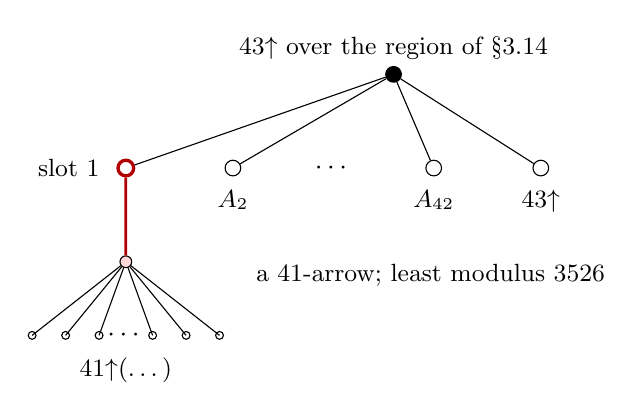
\begin{tikzpicture}[scale=0.85]
  \node[circle,draw,fill=black,inner sep=2pt] (r) at (0,0) {};
  \node[above=2pt] at (0,0) {\small $43\up$ over the region of §3.14};
  \node[circle,draw=red!70!black,line width=1.2pt,inner sep=2pt] (b1) at (-4,-1.4) {};
  \node[circle,draw,inner sep=2pt] (b2) at (-2.4,-1.4) {};
  \node at (-0.9,-1.4) {$\cdots$};
  \node[circle,draw,inner sep=2pt] (b42) at (0.6,-1.4) {};
  \node[circle,draw,inner sep=2pt] (b43) at (2.2,-1.4) {};
  \foreach \b in {b1,b2,b42,b43} \draw (r) -- (\b);
  \node[below=2pt] at (-2.4,-1.5) {\small $A_2$};
  \node[below=2pt] at (0.6,-1.5) {\small $A_{42}$};
  \node[below=2pt] at (2.2,-1.5) {\small $43\up$};
  \node[circle,draw,fill=red!15,inner sep=1.5pt] (n) at (-4,-2.8) {};
  \draw[red!70!black,line width=1pt] (b1) -- (n);
  \foreach \x in {-5.4,-4.9,-4.4,-3.6,-3.1,-2.6} {
    \node[circle,draw,inner sep=1pt] at (\x,-3.9) {};
    \draw (n) -- (\x,-3.9);
  }
  \node at (-4,-3.9) {$\cdots$};
  \node[below=2pt] at (-4,-4.0) {\small $41\up(\dots)$};
  \node[anchor=east] at (-4.25,-1.4) {\small slot $1$};
  \node[anchor=west] at (-2.2,-3.0) {\small a $41$-arrow; least modulus $3526$};
\end{tikzpicture}
\caption{The root of §3.14 after the change. Only the input in slot $1$ is replaced. Its first level now holds a
$41$-arrow over the region, and the family of modulus $43$ keeps only its deeper levels.}\label{fig:nest}
\end{figure}

\subsection*{Refilling slot 1 elsewhere}
The family we cut back had also carried slot $1$ of every copy of $43\up$ nested inside later sections. There are
$264$ such copies: $2$ in §3.15, $1$ in §3.16, $3$ in §3.17, $76$ and $152$ in the $61$- and $67$-arrows of §3.18,
and $15$ in each of the $71$- and $73$-arrows of §3.19. We fill each one with the first set that is an input of some
arrow of the same section, is not already an input of that copy, and repeats no modulus of the system. This adds
$1{,}183$ families. One more copy, at input $80$ of the $83$-arrow of §3.20, takes a set of two families.

These fills cover what the removed family carried explicitly, but not everything it carried implicitly. Several
inputs of the $67$-arrow of §3.18 and the $73$-arrow of §3.19 are sets that are complete only because some of their
own slots are carried, and inside $1 \bmod 43$ those slots had been carried by the removed family. An exact census
lists what remains: $1{,}282$ pieces, about $9.5\cdot10^{-9}$ of the integers. They lie in sixteen $67$-slots ($34$,
$35$, $36$, $39$, $50$, $51$, $53$, $56$--$60$, $63$--$66$) and six $73$-slots ($57$, $62$, $63$, $66$, $69$,
$70$), all in $6 \bmod 8$ and $0 \bmod 3$. None of them lies in the fresh roots of §\ref{sec:roots}.

\subsection*{The Primes 179 through 211}
We first ran the local repairs described below. In seven of the $67$-slots they ran out of
room, and each of these slots gets a fresh root over the piece
$54 \bmod 120\,\cap\,1 \bmod 43\,\cap\,\{\text{$67$-lead } j\}$. Such a piece holds $254$ separated covers (measured
at $179$), enough for any root up to $211$. We use the seven primes from $179$ to $211$
(Table~\ref{tab:roots44}).

\begin{table}[ht]
\centering
\caption{The seven fresh roots of the step to $44$.}\label{tab:roots44}
\begin{tabular}{@{}lccccccc@{}}
\toprule
root prime $q$ & $179$ & $181$ & $191$ & $193$ & $197$ & $199$ & $211$\\
$67$-slot $j$ & $34$ & $50$ & $60$ & $39$ & $36$ & $66$ & $63$\\
families & $3{,}312$ & $3{,}996$ & $6{,}484$ & $9{,}772$ & $13{,}732$ & $13{,}812$ & $23{,}316$\\
\bottomrule
\end{tabular}
\end{table}

\subsection*{Local repairs}
Everything else is closed by the repair loop of §\ref{sec:census}. The target is $1 \bmod 43$, and the cover is the
whole system with the repairs made so far. Each counterexample is traced through the arrows to the input position
that should have covered it. That position then receives the first of two kinds of patch that contains the
counterexample and repeats no modulus.
\begin{enumerate}
\item A \emph{thin family}: the position's context times the class $1 \bmod 43$ and the pins of the region.
\item A \emph{local arrow} $r\up$ on a prime $r$ that the system already uses, placed inside the context. Every one
  of its families carries the whole context, including the $43$-lead and the $67$- or $73$-lead of the position. So
  only families involving $r$ and all of the context's primes can collide with it, and deep inside a context there
  is room even for $r=11$.
\end{enumerate}
The loop ended after $110$ patches, when the formula became unsatisfiable. They were $15$ thin families and $95$ local
arrows: $89$ on the prime $11$, two each on $23$ and $41$, and one each on $17$ and $19$. That is $1{,}801$ families
in all, the smallest of modulus $316{,}910=2\cdot5\cdot11\cdot43\cdot67$.

\subsection*{The system}
The final system has $618{,}413$ families on the $47$ primes up to $211$. Every integer from $44$ to $160$ except $121$
is used as a modulus exactly once. The smallest modulus, $44$, belongs to the family
$\{1 \bmod 4\}\cdot\ray(11,[1,\infty),0,1)$ of §3.5. As in \cite{Nielsen09}, the rays are cut off at a finite depth
and what remains is covered with the help of an auxiliary prime, here $223$. This proves Theorem~\ref{thm:44}; the
details are in \cite{Companion}.

\section{A remark on 45}\label{sec:45}

We do not know whether these methods reach $45$. That would require giving up the modulus $44$ as well, which
belongs to the family $\{1 \bmod 4\}\cdot\ray(11,[1,\infty),0,1)$ of §3.5.

\section*{Acknowledgments}
The search, the exact checks and much of the bookkeeping behind these constructions were carried out with extensive
assistance from Claude, an AI model developed by Anthropic, working under the author's direction.

\begin{thebibliography}{99}

\bibitem{BBMST22} P.~Balister, B.~Bollobás, R.~Morris, J.~Sahasrabudhe and M.~Tiba, \emph{On the Erdős covering
problem: the density of the uncovered set}, Invent. Math. \textbf{228} (2022), 377--414.

\bibitem{CaDiCaL} A.~Biere, K.~Fazekas, M.~Fleury and M.~Heisinger, \emph{CaDiCaL, Kissat, Paracooba, Plingeling and
Treengeling entering the SAT Competition 2020}, Proc. SAT Competition 2020.

\bibitem{Choi71} S.~L.~G.~Choi, \emph{Covering the set of integers by congruence classes of distinct moduli}, Math.
Comp. \textbf{25} (1971), 885--895.

\bibitem{Churchhouse68} R.~F.~Churchhouse, \emph{Covering sets and systems of congruences}, in: Computers in
Mathematical Research, North-Holland, Amsterdam, 1968, 20--36.

\bibitem{Erdos50} P.~Erdős, \emph{On integers of the form $2^k+p$ and some related problems}, Summa Brasil. Math.
\textbf{2} (1950), 113--123.

\bibitem{FFKPY07} M.~Filaseta, K.~Ford, S.~Konyagin, C.~Pomerance and G.~Yu, \emph{Sieving by large integers and
covering systems of congruences}, J. Amer. Math. Soc. \textbf{20} (2007), 495--517.

\bibitem{Gibson09} D.~J.~Gibson, \emph{A covering system with least modulus 25}, Math. Comp. \textbf{78} (2009),
1127--1146.

\bibitem{Hough15} R.~Hough, \emph{Solution of the minimum modulus problem for covering systems}, Ann. of Math. (2)
\textbf{181} (2015), 361--382.

\bibitem{Krukenberg71} C.~E.~Krukenberg, \emph{Covering sets of the integers}, Ph.D. thesis, University of Illinois
at Urbana-Champaign, 1971.

\bibitem{Companion} G.~MacKenzie, \emph{A covering system with minimum modulus 44}, 2026.

\bibitem{Morikawa81a} R.~Morikawa, \emph{On a method to construct covering sets}, Bull. Fac. Liberal Arts Nagasaki
Univ. \textbf{22} (1981), no.~1, 1--11.

\bibitem{Morikawa81b} R.~Morikawa, \emph{Some examples of covering sets}, Bull. Fac. Liberal Arts Nagasaki Univ.
\textbf{21} (1981), no.~2, 1--4.

\bibitem{Nielsen09} P.~P.~Nielsen, \emph{A covering system whose smallest modulus is 40}, J. Number Theory
\textbf{129} (2009), 640--666.

\bibitem{Owens14} T.~E.~Owens, \emph{A covering system with minimum modulus 42}, Master's thesis, Brigham Young
University, 2014.

\bibitem{DRATtrim} N.~Wetzler, M.~J.~H.~Heule and W.~A.~Hunt~Jr., \emph{DRAT-trim: efficient checking and trimming
using expressive clausal proofs}, in: SAT 2014, Lecture Notes in Comput. Sci. \textbf{8561}, Springer, 2014,
422--429.

\end{thebibliography}

\end{document}
